\documentclass[border=15pt,tikz]{standalone}
\usepackage{tikz}
\usetikzlibrary{shapes,arrows,positioning,calc}

\begin{document}

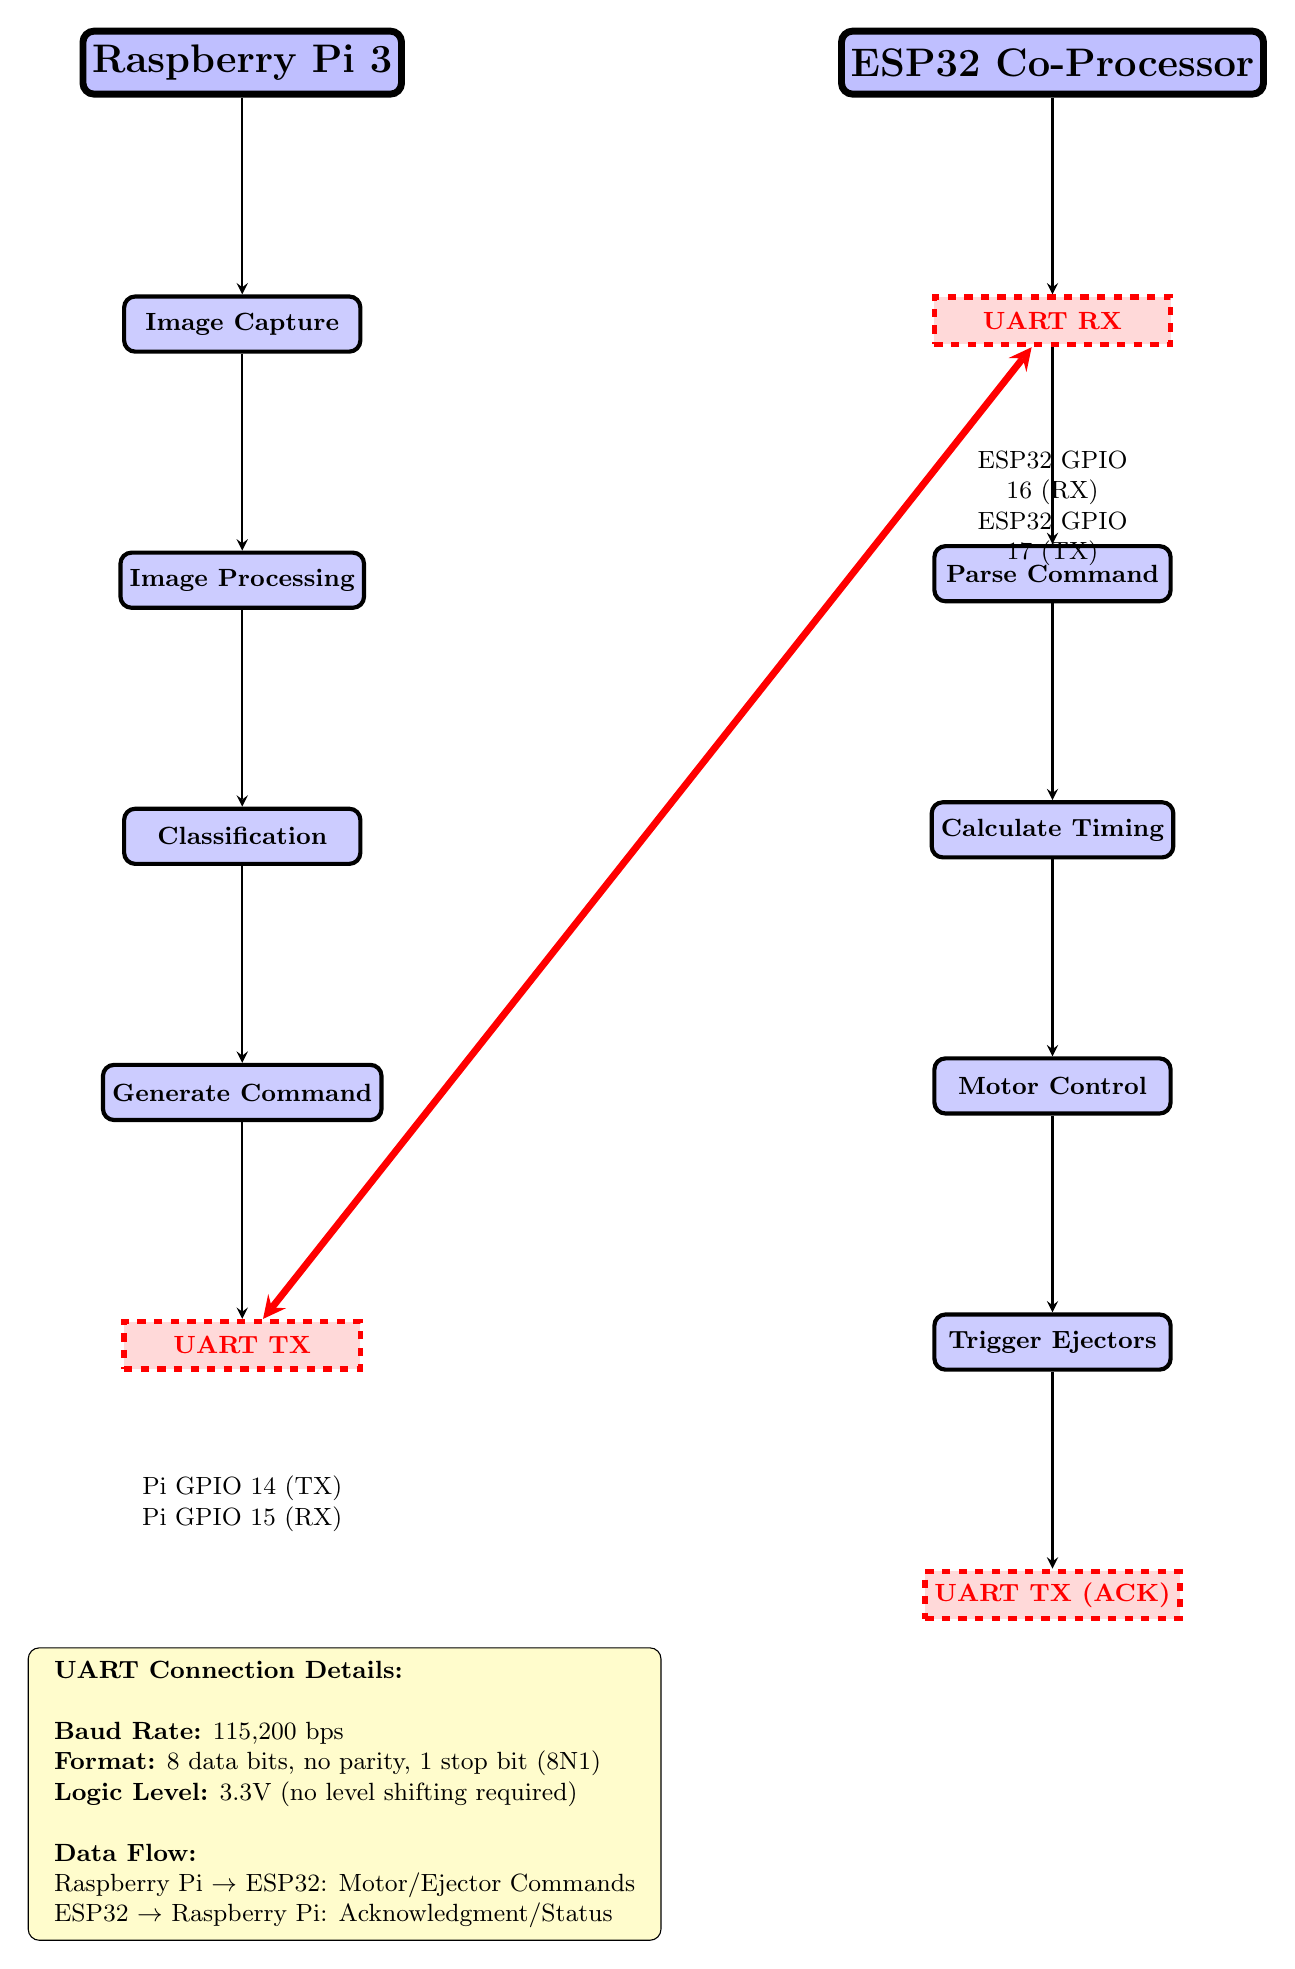
\begin{tikzpicture}[node distance=2.5cm, auto]

% Define styles
\tikzstyle{processor} = [rectangle, rounded corners, minimum width=3.5cm, minimum height=0.8cm, text centered, draw=black, fill=blue!25, line width=2.5pt, font=\bfseries\Large]
\tikzstyle{operation} = [rectangle, rounded corners, minimum width=3cm, minimum height=0.7cm, text centered, draw=black, fill=blue!20, line width=1.5pt, font=\small\bfseries]
\tikzstyle{uart_box} = [rectangle, minimum width=3cm, minimum height=0.6cm, text centered, draw=red, fill=red!15, dashed, line width=2pt, font=\small\bfseries]
\tikzstyle{arrow} = [thick, ->, >=stealth]
\tikzstyle{uart_arrow} = [thick, <->, >=stealth, color=red, line width=2.5pt]

% Raspberry Pi side
\node (pi_title) [processor] {Raspberry Pi 3};
\node (pi_1) [operation, below=of pi_title] {Image Capture};
\node (pi_2) [operation, below=of pi_1] {Image Processing};
\node (pi_3) [operation, below=of pi_2] {Classification};
\node (pi_4) [operation, below=of pi_3] {Generate Command};
\node (pi_tx) [uart_box, below=of pi_4, text=red] {UART TX};

% Connect Pi operations
\draw [arrow] (pi_title) -- (pi_1);
\draw [arrow] (pi_1) -- (pi_2);
\draw [arrow] (pi_2) -- (pi_3);
\draw [arrow] (pi_3) -- (pi_4);
\draw [arrow] (pi_4) -- (pi_tx);

% ESP32 side
\node (esp_title) [processor, right=5.5cm of pi_title] {ESP32 Co-Processor};
\node (esp_rx) [uart_box, below=of esp_title, text=red] {UART RX};
\node (esp_1) [operation, below=of esp_rx] {Parse Command};
\node (esp_2) [operation, below=of esp_1] {Calculate Timing};
\node (esp_3) [operation, below=of esp_2] {Motor Control};
\node (esp_4) [operation, below=of esp_3] {Trigger Ejectors};
\node (esp_tx) [uart_box, below=of esp_4, text=red] {UART TX (ACK)};

% Connect ESP32 operations
\draw [arrow] (esp_title) -- (esp_rx);
\draw [arrow] (esp_rx) -- (esp_1);
\draw [arrow] (esp_1) -- (esp_2);
\draw [arrow] (esp_2) -- (esp_3);
\draw [arrow] (esp_3) -- (esp_4);
\draw [arrow] (esp_4) -- (esp_tx);

% UART Communication
\draw [uart_arrow] (pi_tx) -- (esp_rx);

% GPIO Pin labels
\node [below=1.2cm of pi_tx, font=\small, text width=3cm, text centered] {
Pi GPIO 14 (TX) \\
Pi GPIO 15 (RX)
};

\node [below=1.2cm of esp_rx, font=\small, text width=3cm, text centered] {
ESP32 GPIO 16 (RX) \\
ESP32 GPIO 17 (TX)
};

% Connection info box
\node [draw=black, fill=yellow!20, rounded corners, minimum width=8cm, minimum height=2.5cm, below=3.5cm of pi_tx, xshift=1.3cm, font=\small] {
\begin{tabular}{l}
\textbf{UART Connection Details:} \\
\\
\textbf{Baud Rate:} 115,200 bps \\
\textbf{Format:} 8 data bits, no parity, 1 stop bit (8N1) \\
\textbf{Logic Level:} 3.3V (no level shifting required) \\
\\
\textbf{Data Flow:} \\
Raspberry Pi $\rightarrow$ ESP32: Motor/Ejector Commands \\
ESP32 $\rightarrow$ Raspberry Pi: Acknowledgment/Status
\end{tabular}
};

\end{tikzpicture}

\end{document}
